\section{Evaluation}
\label{sec:Evaluation}
This section is structured as, for each experiment and setup a detailed explanation and motivation on how and why the experiment is needed followed by the results of that experiment. The experiments are motivated by gathering as much information and results as possible to answer the research questions. The first subsection~\ref{sec:simulated_results} will present the results from experiments with synthetic data where a reference image is available. The second subsection~\ref{sec:eval_spc} will present the result from images reconstructed from the SPC. No perfect reference image is available in those experiments therefore the images will be evaluated against near optimal image, no reference QA and against a state of the art SWIR camera. 



\subsection{Simulated results}
\label{sec:simulated_results}
In this section the results produces was simulated by using the reconstructing algorithm and measurement matrix described in section~\ref{sec:TV} and \ref{sec:SOWHMM} on high quality images captured with a state of the art SWIR camera. The images captured by the SWIR camera acts as a ideal reference to the reconstructed images. By simulating the result from "ideal" images the reconstruction process gets a benchmark independent of the SPC.


\subsubsection{Reconstruction performance using reference image}
\label{sec:reconstruction_performance}
In these simulation 21 images captured with a state of the art SWIR camera was reconstructed, the performance of the reconstruction was calculated using PSNR and SSIM. Different degree of noise was added to the signal vector to simulate noise from the SPC where the largest added noise could not reconstruct the image. The test also simulates different under sampling ratios $\frac{M}{N}$ ranging from 5\% to 30\%. 

White gaussian noise with standard deviation $\sigma$ ranging from $0-0.2$ was added to the normalized measurement vector. The limit of $0.2$ standard deviation was set where the most reconstructed images was to degenerate 

\begin{figure}[H]
\raggedright
\begin{minipage}[h]{0.245\textwidth}
    \includegraphics[width=1\textwidth]{result/noisy/1.png}
    \subcaption{Refrence image}
    \label{fig:noise_ref}
\end{minipage}\linebreak
\begin{minipage}[t]{0.245\textwidth}
    \includegraphics[width = \textwidth]{result/noisy/1_5_20.png}
    \subcaption{$\frac{M}{N} = 5\% \text{, } \sigma = 0.2$}
    \label{fig:noise_5_20}
    \includegraphics[width = \textwidth]{result/noisy/1_5_12.png}
    \subcaption{$\frac{M}{N} = 5\% \text{, } \sigma = 0.12$}
    \label{fig:noise_5_12}
        \includegraphics[width = \textwidth]{result/noisy/1_5_6.png}
    \subcaption{$\frac{M}{N} = 5\% \text{, } \sigma = 0.06$}
    \label{fig:noise_5_12}
    \includegraphics[width = \textwidth]{result/noisy/1_5_0.png}
    \subcaption{$\frac{M}{N} = 5\%$}
    \label{fig:noise_5_12}
\end{minipage}
\begin{minipage}[t]{0.245\textwidth}
    \includegraphics[width = \textwidth]{result/noisy/1_15_20.png}
    \subcaption{$\frac{M}{N} = 15\% \text{, } \sigma = 0.2$}
    \label{fig:noise_15_20}
    \includegraphics[width = \textwidth]{result/noisy/1_15_12.png}
    \subcaption{$\frac{M}{N} = 15\% \text{, } \sigma = 0.12$}
    \label{fig:noise_15_12}
    \includegraphics[width = \textwidth]{result/noisy/1_15_6.png}
    \subcaption{$\frac{M}{N} = 15\% \text{, } \sigma = 0.06$}
    \label{fig:noise_15_6}
    \includegraphics[width = \textwidth]{result/noisy/1_15_0.png}
    \subcaption{$\frac{M}{N} = 15\%$}
    \label{fig:noise_15_0}
\end{minipage}
\begin{minipage}[t]{0.245\textwidth}
    \includegraphics[width = \textwidth]{result/noisy/1_20_20.png}
    \subcaption{$\frac{M}{N} = 20\% \text{, } \sigma = 0.2$}
    \label{fig:noise_20_20}
    \includegraphics[width = \textwidth]{result/noisy/1_20_12.png}
    \subcaption{$\frac{M}{N} = 20\% \text{, } \sigma = 0.12$}
    \label{fig:noise_20_12}
    \includegraphics[width = \textwidth]{result/noisy/1_20_6.png}
    \subcaption{$\frac{M}{N} = 20\% \text{, } \sigma = 0.06$}
    \label{fig:noise_20_6}
    \includegraphics[width = \textwidth]{result/noisy/1_20_0.png}
    \subcaption{$\frac{M}{N} = 20\%$}
    \label{fig:noise_20_0}
\end{minipage}
\begin{minipage}[t]{0.245\textwidth}
    \includegraphics[width = \textwidth]{result/noisy/1_30_20.png}
    \subcaption{$\frac{M}{N} = 30\% \text{, } \sigma = 0.2$}
    \label{fig:noise_30_20}
    \includegraphics[width = \textwidth]{result/noisy/1_30_12.png}
    \subcaption{$\frac{M}{N} = 30\% \text{, } \sigma = 0.12$}
    \label{fig:noise_30_12}
    \includegraphics[width = \textwidth]{result/noisy/1_30_6.png}
    \subcaption{$\frac{M}{N} = 30\% \text{, } \sigma = 0.06$}
    \label{fig:noise_30_6}
    \includegraphics[width = \textwidth]{result/noisy/1_30_0.png}
    \subcaption{$\frac{M}{N} = 30\%$}
    \label{fig:noise_30_0}
\end{minipage}
\end{figure}

\begin{figure}[H]
    \centering
    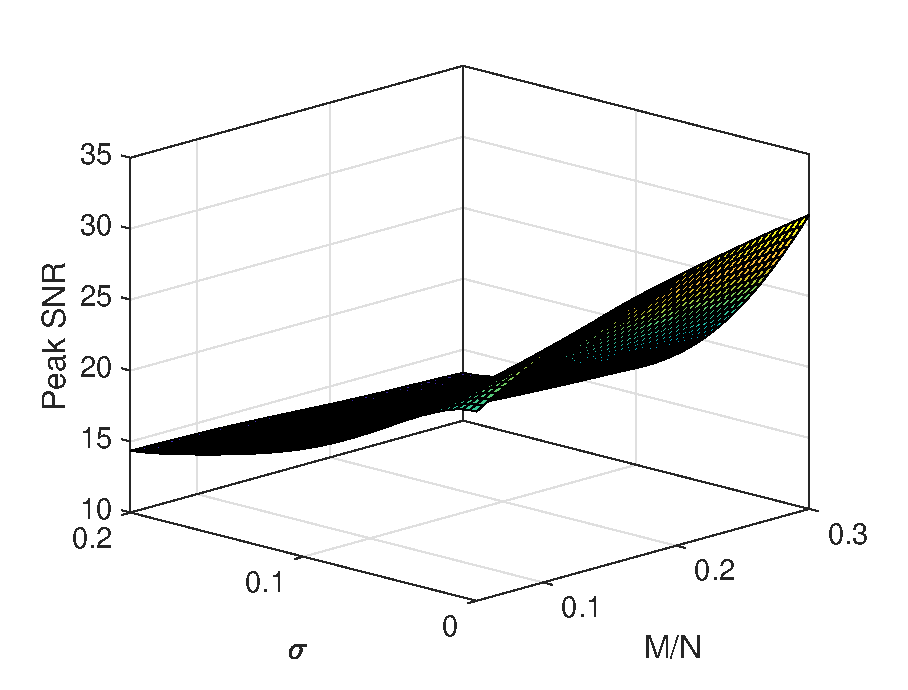
\includegraphics[width = 0.7\linewidth]{result/synt_sss/PSNR_fit.eps}
    \caption{Peak SNR result depending on number of measurements and simulated noise level.}
    \label{fig:psnr_3d}
\end{figure}
\todo[inline]{Change to dB}

\begin{figure}[H]
    \centering
    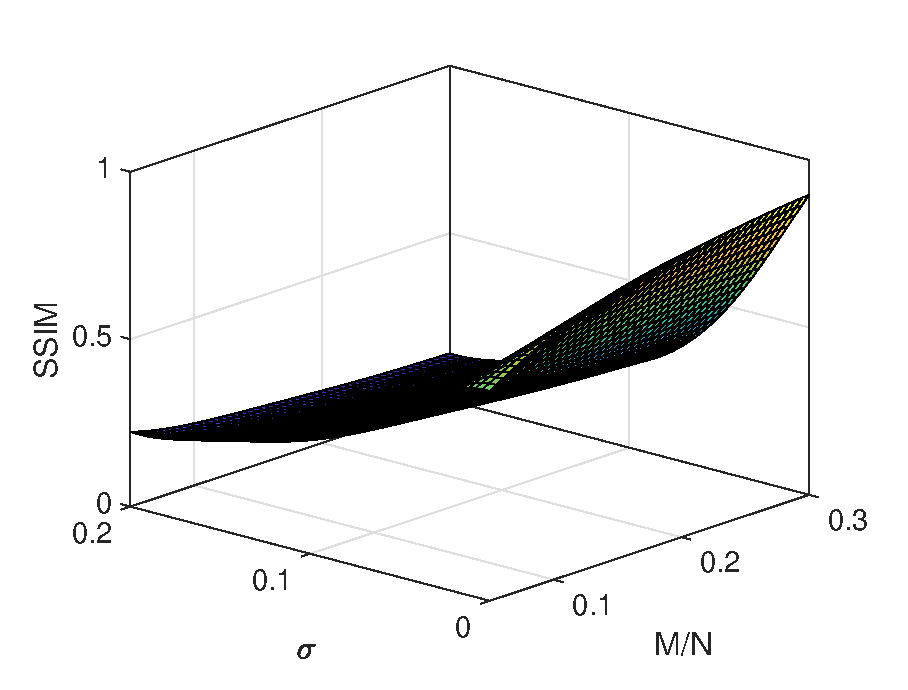
\includegraphics[width = 0.7\linewidth]{result/synt_sss/SSIM_fit.eps}
    \caption{SSIM result depending on number of measurements and simulated noise level.}
    \label{fig:ssim_3d}
\end{figure}

In figure~\ref{fig:psnr_3d} and \ref{fig:ssim_3d} the reconstruction performance is presented in PSNR and SSIM score respectively. The reconstitution performance is increased when the under sampling ratio is increased and when the noise is decreased.  

\subsubsection{Reconstruction performance using no reference quality assessment}
BRISQUE lower score is better.

\begin{figure}[H]
    \centering
    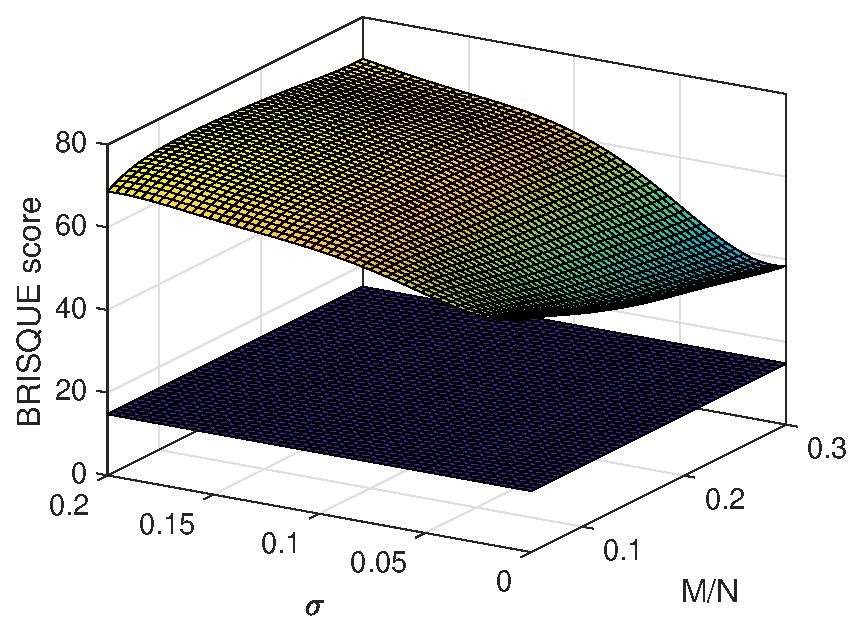
\includegraphics[width = 0.7\linewidth]{result/synt_brisque/BRISQUE_fit.eps}
    \caption{BRISQUE result depending on number of measurements and simulated noise level. Lower surface is reference image score.}
    \label{fig:Brisque_3d}
\end{figure}

\begin{figure}[H]
    \centering
    \includegraphics[width = 0.95\linewidth]{result/synt_brisque/Brisque_fit_flat3.eps}
    \caption{BRISQUE result depending on number of measurements for different simulated noise levels.}
    \label{fig:Brisque_2d}
\end{figure}
\todo[inline]{Add "optimal performance into the graph"}







